
\graphicspath{{./Figs/}}

\chapter{Background} 
This chapter outlines the core theory and topics relevant for optimising MAVs and relevant literature regarding the effect of propeller interactions on MAVs. Crucial coefficients, concepts and terminology are explained here. This section will cover general aircraft geometry, aerodynamic forces, reference frames, longitudinal stability, lateral stability and Reynolds number. 

\section{Aircraft Geometry}
Several aircraft geometric parameters will be referred to throughout this thesis. Key parameters discussed are the wingspan, chord length, aspect ratio, sweep, dihedral and twist. Figure \ref{fig:aircraftgeometry} shows some of these.

\begin{figure}[H]
% \hspace*{-1.3in}
  \centering
   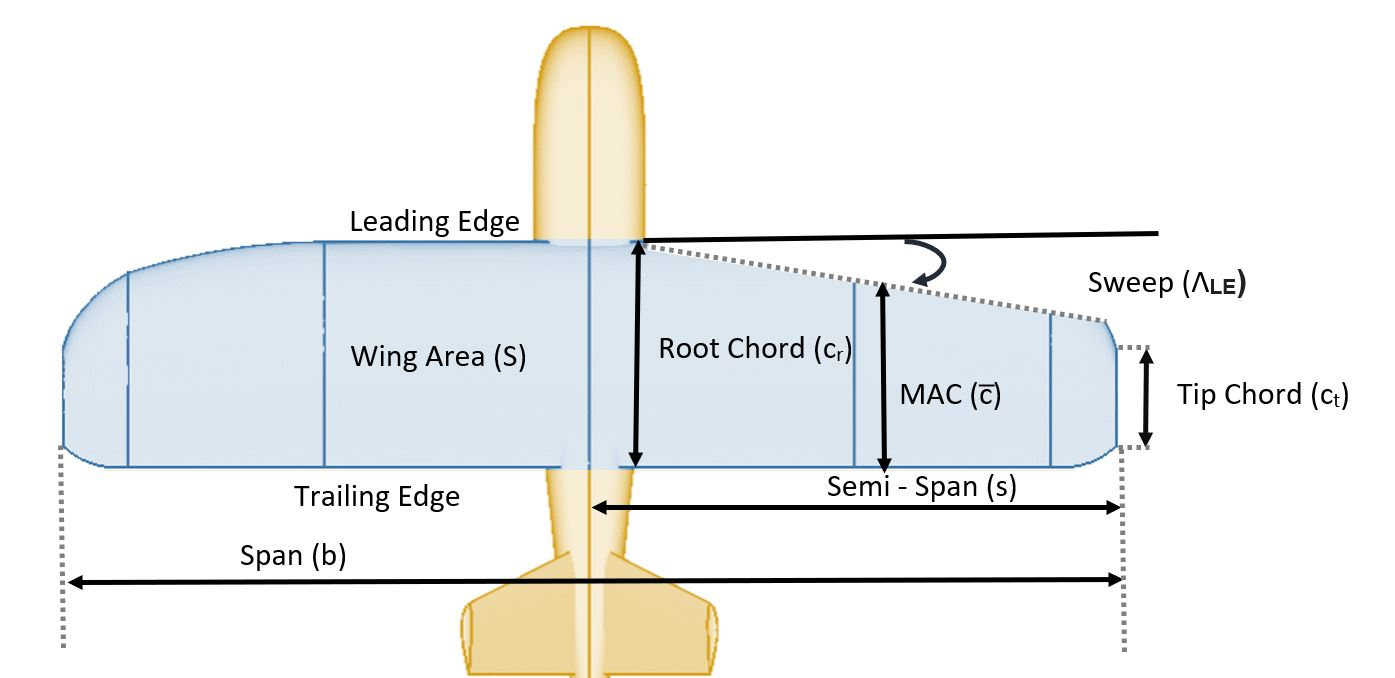
\includegraphics[width=1\linewidth]{03_LiteratureReview/Figs/geometry.JPG}
  \caption{Aircraft geometric parameters}
  \label{fig:aircraftgeometry}
\end{figure}

\section{Span}
The wingspan ($b$) is the distance from one wing tip to the other. The semi-span (s) is the distance from the fuselage reference line to the wing tip. These parameters are also shown in Figure \ref{fig:aircraftgeometry}. 

\section{Chord}
The chord is the distance between the leading and trailing edge of the wings shown in Figure \ref{fig:aircraftgeometry}. The chord is often defined in terms of three main parameters, these are:

\begin{itemize}
    \item \textbf{Root Chord (denoted $c_r$):} This is the chord length where the wing meets the fuselage and is generally the position where the chord length is the longest. 
    \item \textbf{Tip Chord (denoted $c_t$):} The tip chord is the chord length at the tips of the wings 
    \item \textbf{Mean Aerodynamic Chord (MAC):} The mean aerodynamic chord is used to represent the wing in only two dimensions. The MAC is the chord length at which the resultant aerodynamic force acts. The MAC is defined by Equation \ref{eqn:MAC} and is taken from wing tip to wing tip. In the case of a straight tapered wing with a taper ratio, the MAC equation can be simplified to Equation \ref{eqn:MACSimplified}.
    
\end{itemize} 

\begin{equation}
    \bar{c} =  \frac{ \int_{0}^{b} c(y)^2 dy}{\int_{0}^{b} dy}
    \label{eqn:MAC}
\end{equation}

\begin{equation}
    \bar{c} =  \frac{ 2c_r(1 + \lambda + \lambda^2)}{3(1 + \lambda)}
    \label{eqn:MACSimplified}
\end{equation}

 The taper ratio defines the ratio between the root and tip chord lengths. The taper ratio is given by Equation \ref{eqn:taper}.
 
 \begin{equation}
     \lambda = \frac{c_t}{c_r}
     \label{eqn:taper}
 \end{equation}
 
 The taper ratio is significant as it influences the lift distribution over the wing. By reducing the wing area towards the wing tips, the moment produced by the wings is reduced. 
 
\section{Sweep}
The sweep is the angle ($\Lambda_{LE}$) between the $y_b$ axis and the leading edge. When wings are swept back, the flow is directed outwards along the length of the wing. This also changes the angle of attack towards the wings' tips. A negative sweep angle (generally only seen on experimental aircraft such as the Grumman X-29 shown in Figure \ref{fig:X29}) directs the flow inboard towards the fuselage. Sweep is also used to assist with static longitudinal stability. A positive sweep angle will move the aircraft's centre of gravity backwards and vice versa. The sweep angle ($\Lambda_{LE}$) can be used to fine-tune the pitch stability. Sweep is also used to delay shock wave formation on wings. In this phenomenon, at high Mach numbers ($>$ 0.8), a sharp discontinuity of pressure is seen in a narrow region travelling through a medium. 

\begin{figure}[H]
% \hspace*{-1.3in}
  \centering
   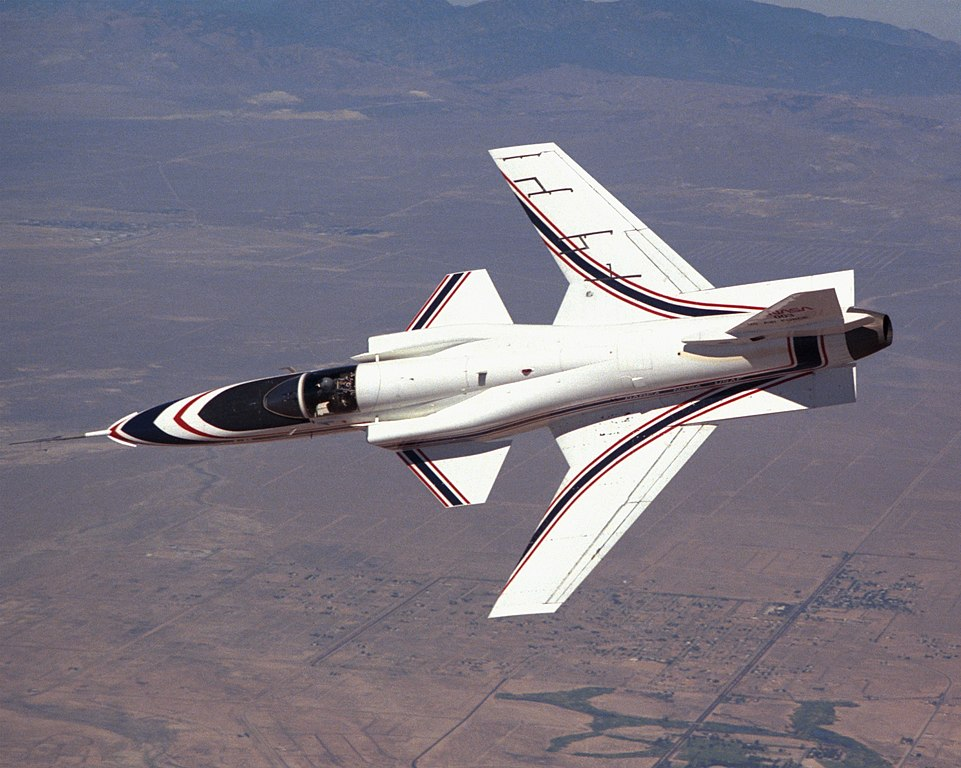
\includegraphics[width=1\linewidth]{03_LiteratureReview/Figs/negativeSweep.jpg}
  \caption{Forward swept wings of Grumman X-29 (negative sweep angle) \cite{plane}}
  \label{fig:X29}
\end{figure}

\section{Dihedral}
The dihedral angle ($\gamma$) is the angle between the wing and the $y_b$ axis, which is represented by the horizontal dotted line in Figure \ref{fig:dihedral}. A dihedral angle is when the wing tip is at a higher point than the root of the wing. This is the opposite for the case of an anhedral angle, also shown in Figure \ref{fig:dihedral}. Having a dihedral angle increases the lateral stability - particularly when banking, as the lower wing will fly at a higher angle of attack than the higher wing. 

\begin{figure}[H]
% \hspace*{-1.3in}
  \centering
   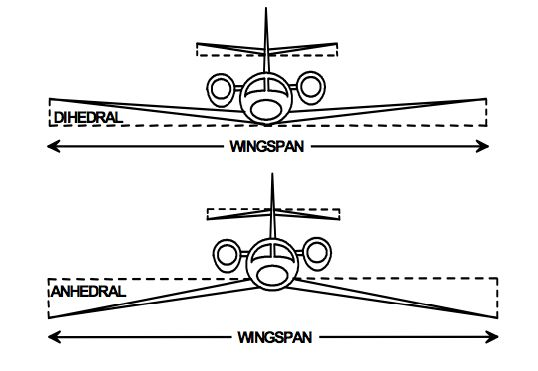
\includegraphics[width=1\linewidth]{03_LiteratureReview/Figs/dihedral.jpg}
  \caption{Wing dihedral and anhedral example. Image source: \cite{moreplane}}
  \label{fig:dihedral}
\end{figure}

\section{Twist and Incidence}
The wing twist angle ($\theta_t$) is the angle between the tip chord reference line and the root chord. By convention, a positive wing twist angle is defined as a downward twist on the wing. Figure \ref{fig:twist} shows an example of this. Another significant parameter is the wing incidence angle ($\theta_i$) which is the angle between the fuselage reference line and the root chord line. In this case, a positive incidence angle is defined as an upward twisted root chord. 

The wing twist is often used to redistribute the lift along the wing's surface. The wing tip is the last wing surface that will experience stall; particularly when in a steep climb or roll manoeuvre. By twisting the wingtip downwards with respect to the rest of the wing, the effective angle of attack will be lower at the wingtip than at the root. This means that the root will stall before the wingtip. This is desirable as control surfaces such as ailerons lose their effectiveness when the wingtips stall first. 


\begin{figure}[H]
% \hspace*{-1.3in}
  \centering
  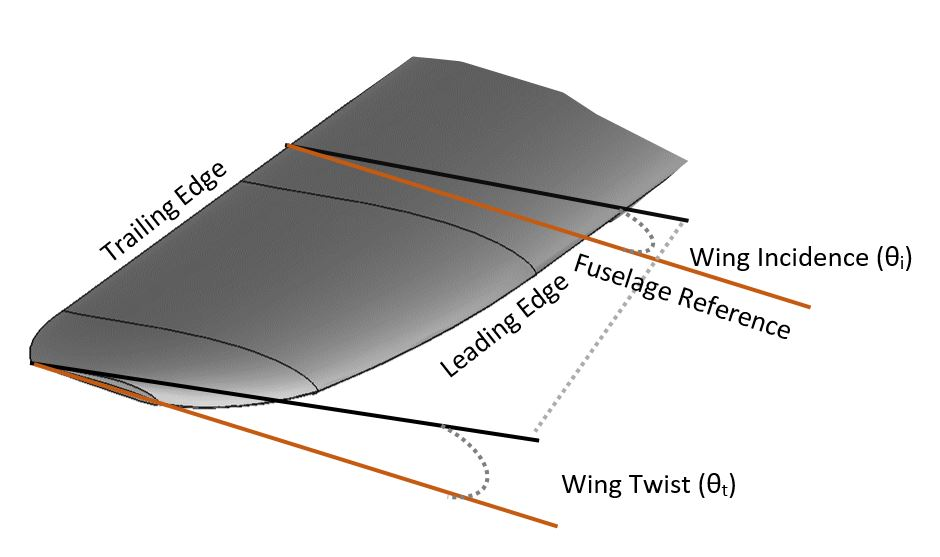
\includegraphics[width=1\linewidth]{02_Background/Figs/wingo.JPG}
  \caption{Wing twist and incidence angle}
  \label{fig:twist}
\end{figure}

\section{Aspect Ratio}
The aspect ratio (AR) is significant when considering an aircraft's aerodynamic efficiency. First, the wing area (S) must be introduced. The AR can be calculated through Equation \ref{eqn:Aspect}.

\begin{equation}
    AR = \frac{b^2}{S}
    \label{eqn:Aspect}
\end{equation}

 Where b is the wing span and S is the total platform area of the wing, also shown in Figure \ref{fig:aircraftgeometry}, as the area coloured blue. 

Higher aspect wings produce less lift-induced drag - however, they often require more structural support and are typically heavier than lower AR aircraft. High aspect wings are long and thin, whilst low aspect wings are short and wide. Figure \ref{fig:AR} shows two aircraft with high and medium ARs. The Schleicher aircraft shown has a much higher AR. This also means it has high aerodynamic efficiency. 



\begin{figure}[H]
% \hspace*{-1.3in}
  \centering
  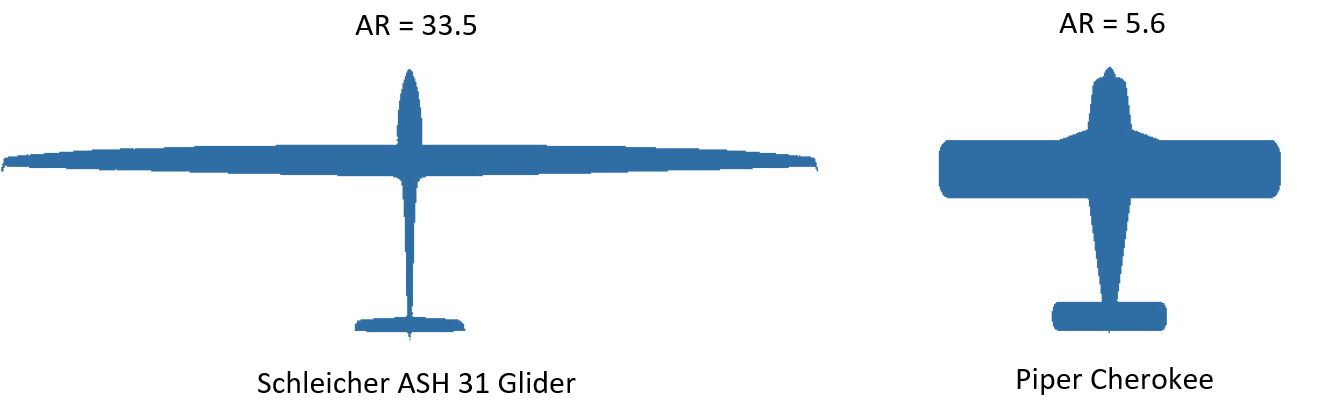
\includegraphics[width=1\linewidth]{03_LiteratureReview/Figs/AspectRatio.JPG}
  \caption{High and medium aspect ratio aircraft examples}
  \label{fig:AR}
\end{figure}

\section{Reference Frames}
The primary reference frames used to describe the position of an aircraft are:
\begin{itemize}
    \item Earth Centered Axes
    \item Local-vertical local-horizontal (LVLH) Axes
    \item Body Axes
    \item Stability Axes
    \item Air Axes
\end{itemize}

Figure \ref{fig:refernce} provides a visualisation to assist with the following explanations.

\begin{figure}[H]
% \hspace*{-1.3in}
  \centering
  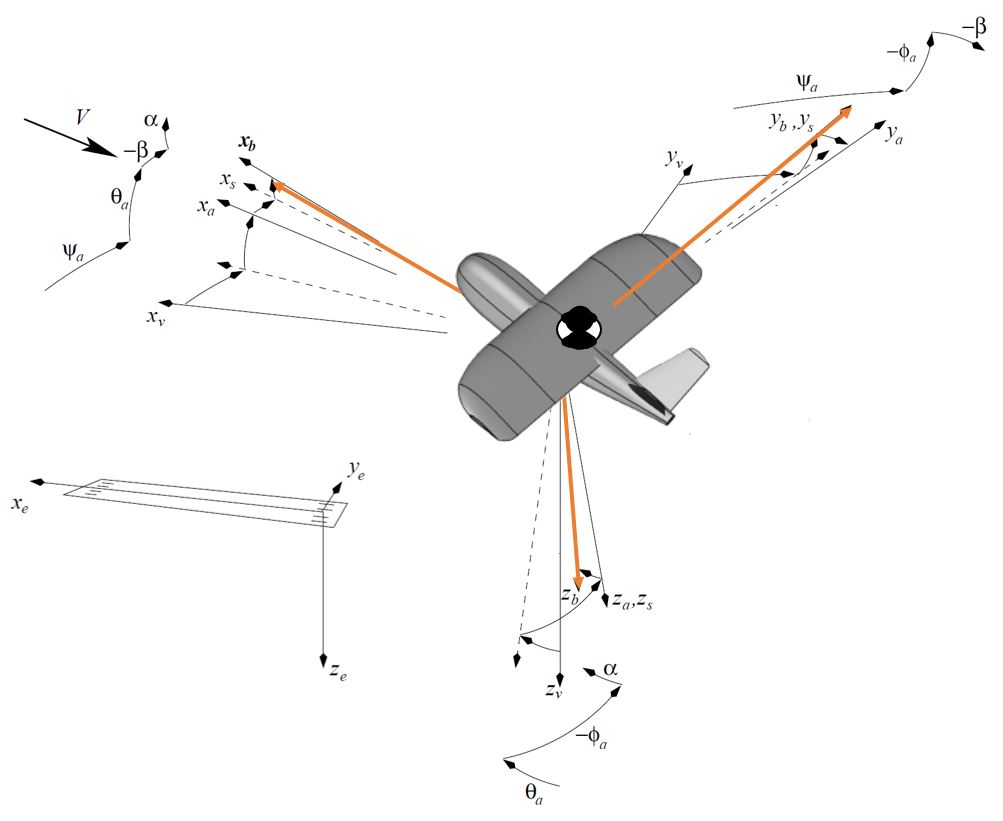
\includegraphics[width=1\linewidth]{03_LiteratureReview/Figs/referenceFrame.JPG}
  \caption{Aircraft reference frames}
  \label{fig:refernce}
\end{figure}

\section{Earth Centered Axes: denoted as \texorpdfstring{($x_e$, $y_e$, $z_e$)}{L}}
The Earth centered axes is a global reference frame with the centre of the Earth's origin. From the Earth's centre, three orthogonal axes remain fixed to the Earth. This axis is primarily used when describing the position of aircraft. Further visualisation of this reference frame is shown in Figure \ref{fig:refernceEarth}. As Earth has an ellipsoid shape (rather than a sphere), the position is described in terms of the latitude ($\phi$), longitude ($\lambda$), and altitude (h).

\begin{figure}[H]
% \hspace*{-1.3in}
  \centering
  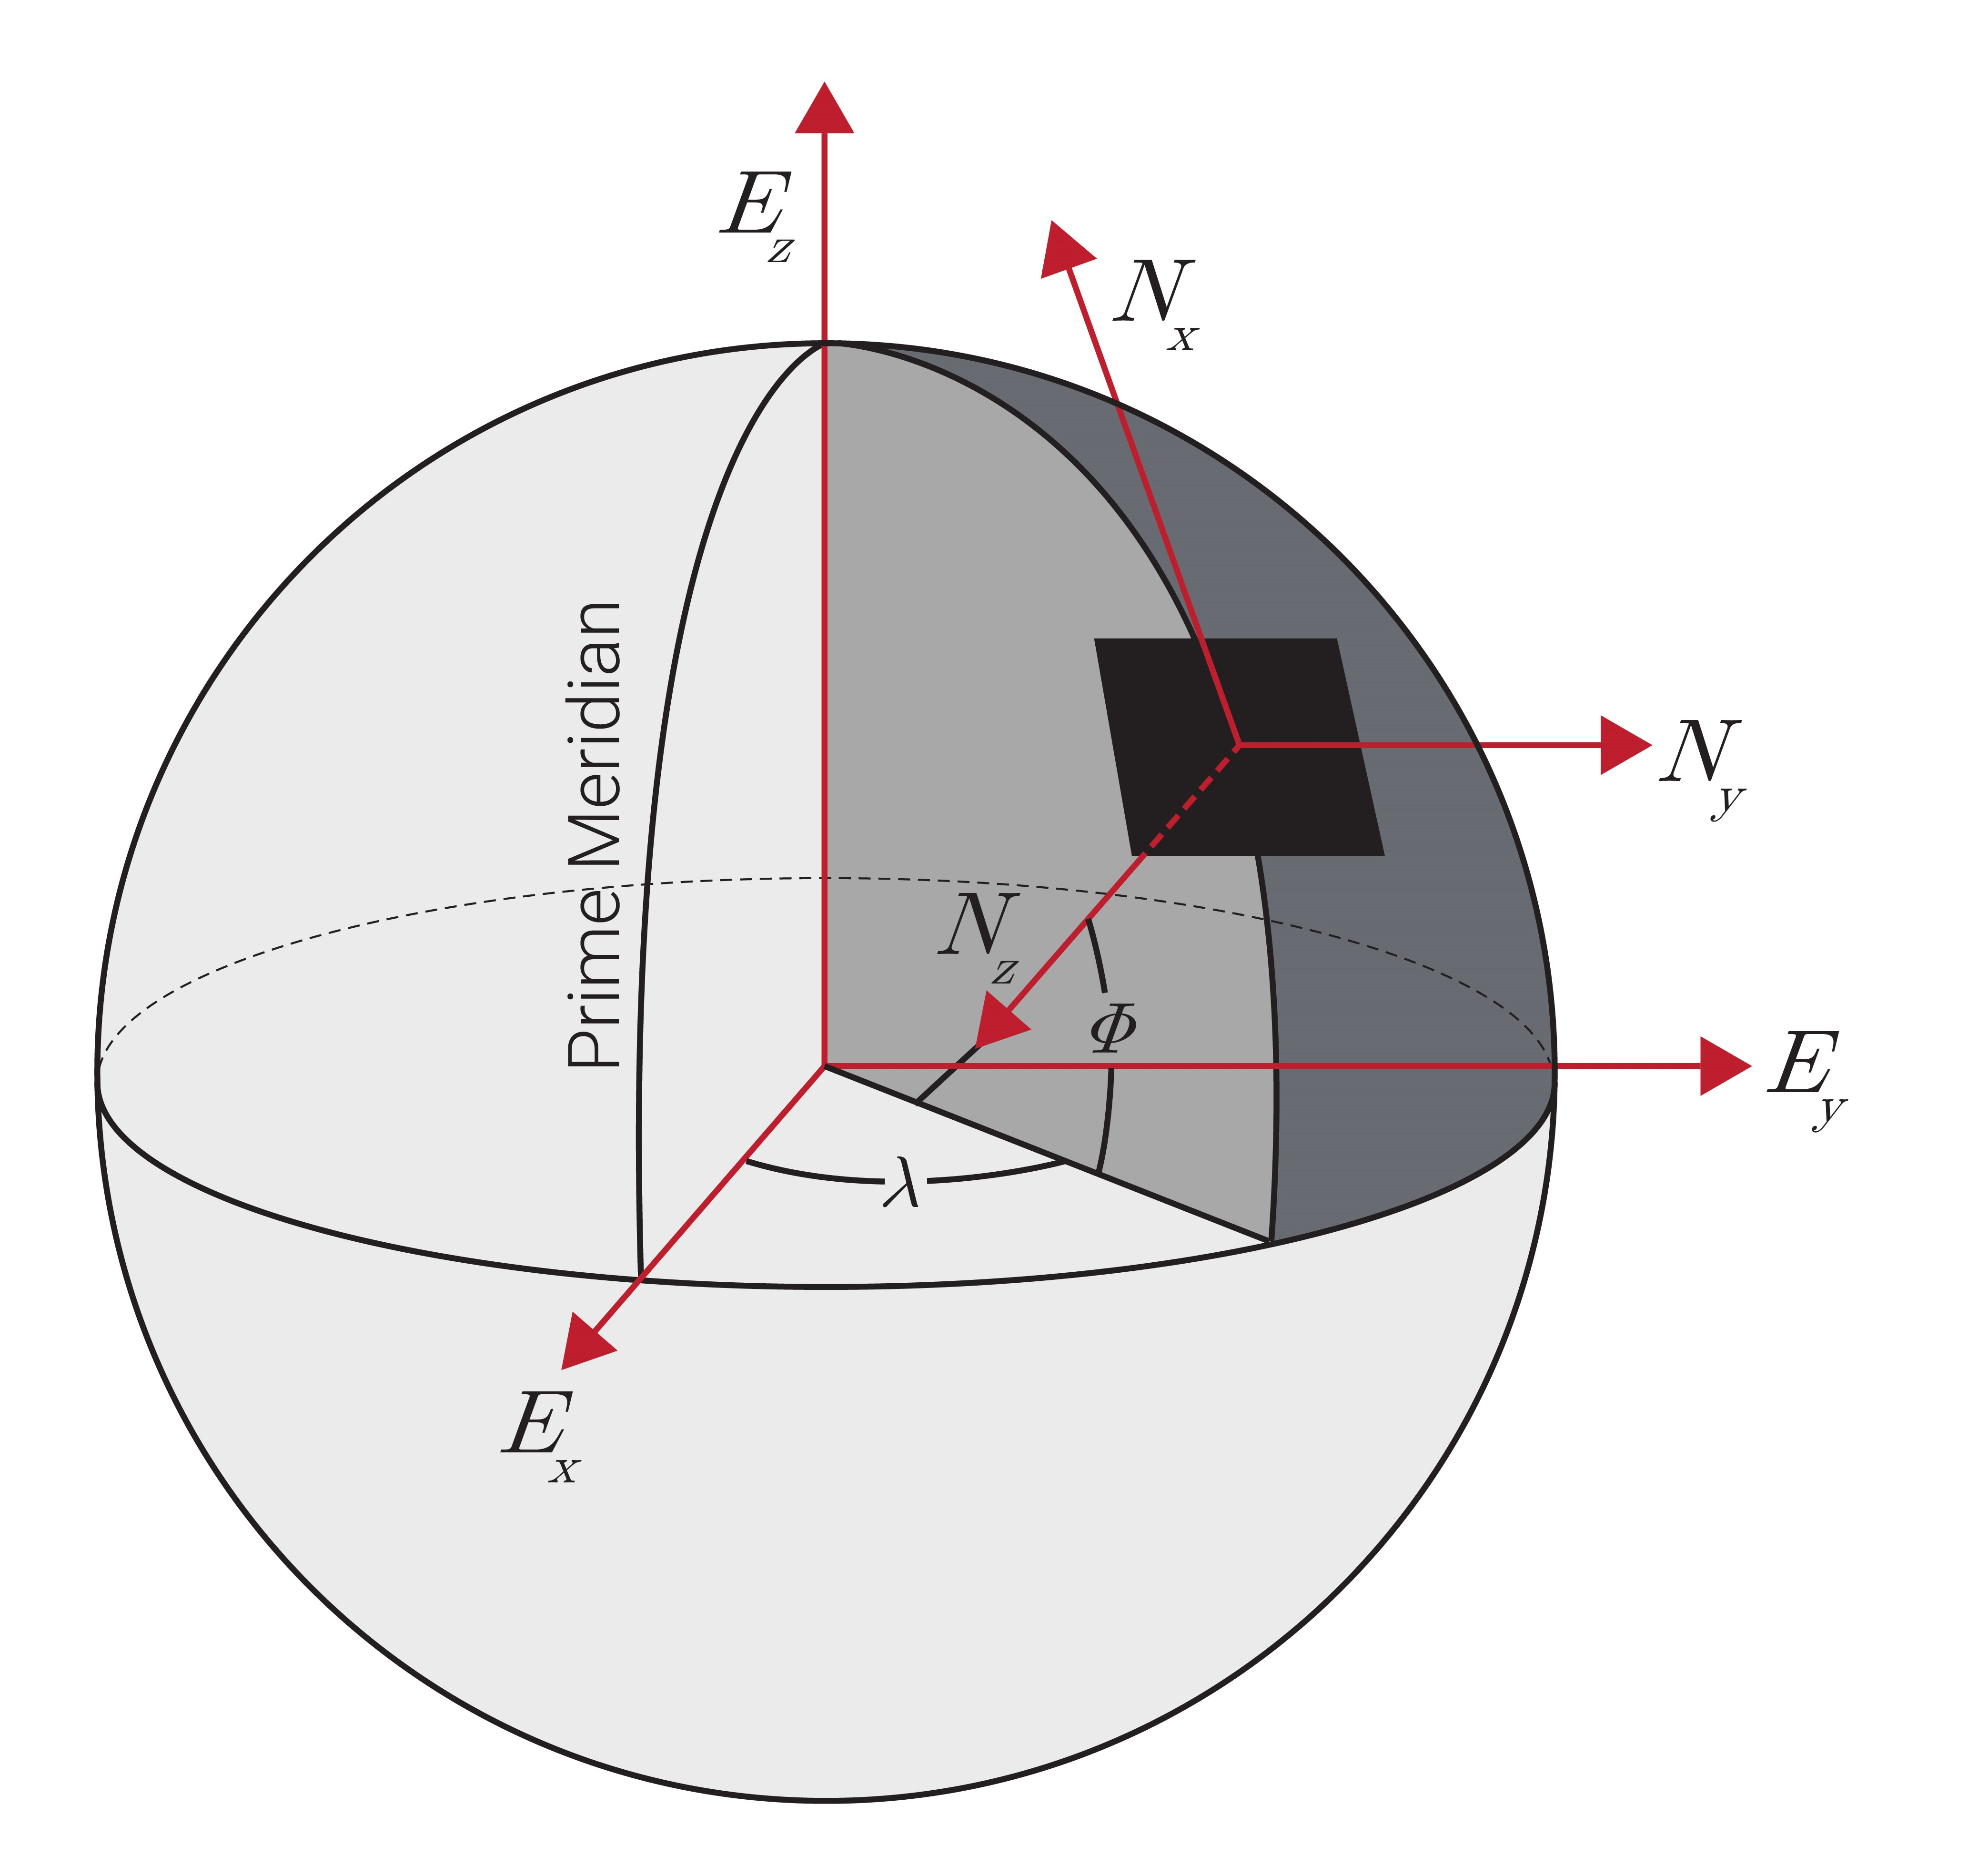
\includegraphics[width=0.7\linewidth]{03_LiteratureReview/Figs/ref_ecef.jpg}
  \caption{Earth centered axes \cite{VectorNAV}}
  \label{fig:refernceEarth}
\end{figure}

\section{LVLH Axes: denoted as \texorpdfstring{($x_v$, $y_v$, $z_v$)}{L}}
 This axis frame translates with the aircraft and is aligned with the Earth axes previously described. It is shown in Figure \ref{fig:refernce}.

\section{Body Axes: denoted as \texorpdfstring{($x_b$, $y_b$, $z_b$)}{L}} 
This axis is positioned at the aircraft's centre of gravity. Figure \ref{fig:refernce} shows this position in the aircraft's centre. The body axes translate with the aircraft and are highlighted in orange in Figure \ref{fig:refernce}.

\section{Stability Axes: denoted as \texorpdfstring{($x_s$, $y_s$, $z_s$)}{L}} 
The stability axis has its origin at the centre of gravity, shown in Figure \ref{fig:refernce}. It translates with the aircraft's movement. $x_s$ aligns with the air path and is described as an offset from $x_b$ by an angle of $\alpha$ (further described in \ref{subsubsec:keyparam}). $y_s$ is aligned with the body axes $y_b$ and $z_s$ acts perpendicular to both $x_s$ and $y_s$.


\section{Air Path Axes: denoted as \texorpdfstring{($x_a$, $y_a$, $z_a$)}{L}}
The air path axis has its origin at the centre of gravity. $x_a$ is aligned with the relative air path and is offset from $x_b$ by the angle of attack ($\alpha$). $y_a$ is also aligned with the relative air path and is offset from the $y_b$ by the sideslip angle ($\beta$). $z_a$ is perpendicular to both $x_a$ and $y_a$. 

\section{Key Parameters}
\label{subsubsec:keyparam}
Some key parameters are used to define the motion of the aircraft. These are explained below: 
\begin{itemize}
    \item \textbf{Aerodynamic Angles ($\alpha, \beta$):} These angles are used to describe the offset of the aircraft's body axes to the relative air path. $\alpha$ is also known as the angle of attack and describes the angle between the $x_a$ and $x_b$ positions. $\beta$ is also known as the side slip angle and describes the angle between the $y_a$ and $y_b$ positions. These angles are also shown in Figure \ref{fig:refernce}.
    \item \textbf{Euler Angles ($\theta_a, \phi_a, \psi_a $):} The Euler angles are used to describe the orientation of rigid bodies with respect to a fixed coordinate system. In the case of aircraft, this describes the pitch ($\theta_a$), yaw ($\psi_a$) and roll ($\phi_a$). These angles are relative to the LVLH reference frame. These can be seen in Figure \ref{fig:refernce}.
\end{itemize}

\section{Aerodynamic Forces and Coefficients}
Airfoils which are designed to produce lift, achieve this by creating a  pressure difference between the upper and lower surface when moving through a fluid. This lift force acts perpendicular to the chord line and is shown in Figure \ref{fig:pressureWing}.



\begin{figure}[H]
     \centering
     \begin{subfigure}[b]{0.45\textwidth}
         \centering
         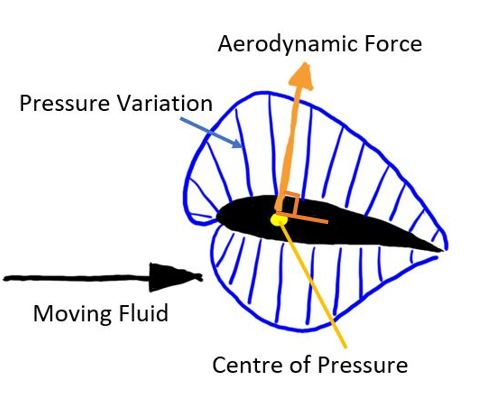
\includegraphics[width=\textwidth]{02_Background/Figs/smol.JPG}
         \caption{Low angle of attack}
         \label{fig:Press2a}
     \end{subfigure}
     \hfill
     \begin{subfigure}[b]{0.45\textwidth}
         \centering
         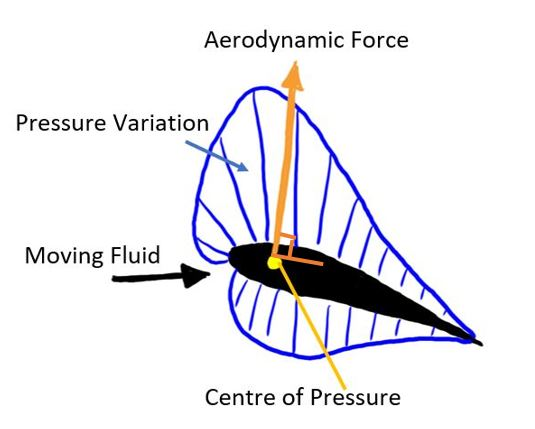
\includegraphics[width=\textwidth]{02_Background/Figs/big.JPG}
         \caption{High angle of attack}
         \label{fig:Press2b}
     \end{subfigure}
     \hfill
        \caption{Pressure distribution over a wing }
        \label{fig:pressureWing}
\end{figure}



In order to simplify calculations regarding this force distribution, the aerodynamic centre is used. The wing's aerodynamic centre is the wing's position where when the net force is applied, the total moment created with respect to the angle of attack remains constant. Through these simplifications, the total force acts through a single point - the aerodynamic centre. The main forces which act on the wing are lift and drag. Lift (L) is the force acting normally on the air path axes ($z_a$). Drag (D) is the force that acts both in the $x_a$, air path axis and long the aircraft surface due to air friction. The main components for the aerodynamic forces and coefficients are the wing, tail and fuselage. The main forces are also shown in Figure \ref{fig:aeroforces}.



\begin{figure}[H]
% \hspace*{-1.3in}
  \centering
  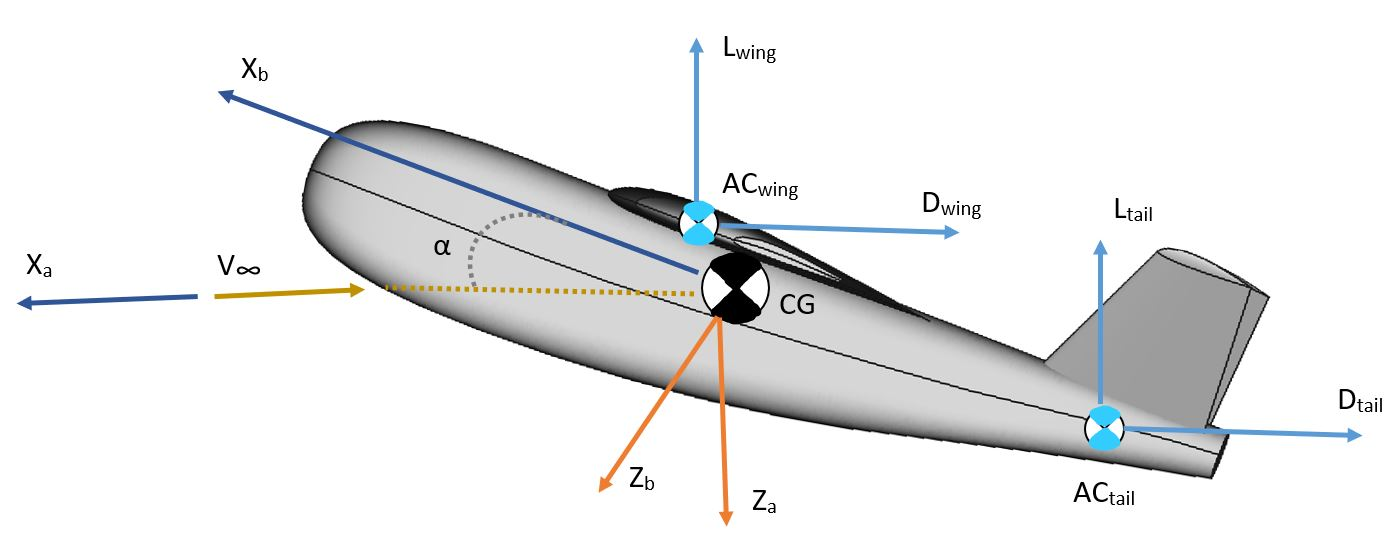
\includegraphics[width=1\linewidth]{03_LiteratureReview/Figs/Aeroforces2.JPG}
  \caption{Aerodynamic forces acting on MAV}
  \label{fig:aeroforces}
\end{figure}
Two significant aerodynamic coefficients are used as the lift and drag forces coefficients shown in Equations \ref{eqn:lift} and \ref{eqn:drag}. These coefficients are the lift and drag forces when normalised by the dynamic pressure (q) and the wing area (S). 


\begin{equation}
    C_L = \frac{L}{qS} = \frac{L}{\frac{1}{2}\rho {V_\infty}^2 S}
    \label{eqn:lift}
\end{equation}

\begin{equation}
     C_D = \frac{D}{qS} = \frac{D}{\frac{1}{2}\rho {V_\infty}^2 S}
     \label{eqn:drag}
\end{equation}

The lift coefficient can also be described in terms of the angle of attack, the lift coefficient at an angle of attack of 0 ($C_{L_0}$) and the slope of the lift curve with respect to the angle of attack ($C_{L_\alpha}$). 

\begin{equation}
    C_L \approx C_{L_0} + C_{L_\alpha}\alpha
    \label{eqn:Cl}
\end{equation}

Figure \ref{fig:Clalpha} shows a visualisation of these parameters. 

\begin{figure}[H]
    \centering
    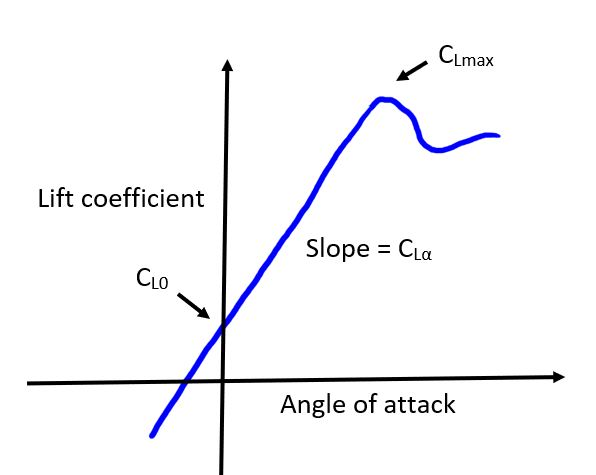
\includegraphics[scale = 0.8]{02_Background/Figs/liftcurveslope.JPG}
    \caption{Lift curve with respect to angle of attack}
    \label{fig:Clalpha}
\end{figure}

Equation \ref{eqn:Cl} is accurate at small angles of attack where the lift curve slope is linear as shown in Figure \ref{fig:Clalpha}. The lift curve slope at higher angles of attack becomes non-linear due to flow separation, and hence Equation \ref{eqn:Cl} is an inaccurate approximation. Drag can be estimated through Equation \ref{eqn:Cd}, where $C_{D_0}$ is the drag due to skin friction and e is the Oswald efficiency factor. The Oswald efficiency factor measures the lift distribution efficiency across a wing. 


\begin{equation}
    C_D \approx C_{D_0} + \frac{{C_L}^2}{\pi ARe}
    \label{eqn:Cd}
\end{equation}



\section{Static Longitudinal Stability}

Static longitudinal stability is determined from the pitching moment M. The pitching moment is defined as shown in Equation \ref{eqn:MACSimplified}.

\begin{equation}
    C_M = \frac{M}{\frac{1}{2}\rho {V_\infty}^2 S \overline{c}}
\end{equation}

The derivative of the pitching moment with respect to the angle of attack must be negative with a positive angle of attack to be stable. This is also given in Equation \ref{eqn:pitching}.

\begin{equation}
    C_{M_\alpha} = \frac{\delta C_M}{\delta \alpha} < 0 
    \label{eqn:pitching}
\end{equation}

The aerodynamic centre of the aircraft is also referred to as the neutral point. The total aerodynamic force acts through the neutral point and is the position where no change in pitching moment is seen with a variation in the angle of attack ($C_{M_\alpha} = 0$ when $x_{cg} = N_0$). Figure \ref{fig:AC} shows the parameters on the aircraft. When the position of the centre of gravity is the same as the neutral point, the aircraft is neutrally stable. 

\begin{figure}[H]
% \hspace*{-1.3in}
  \centering
   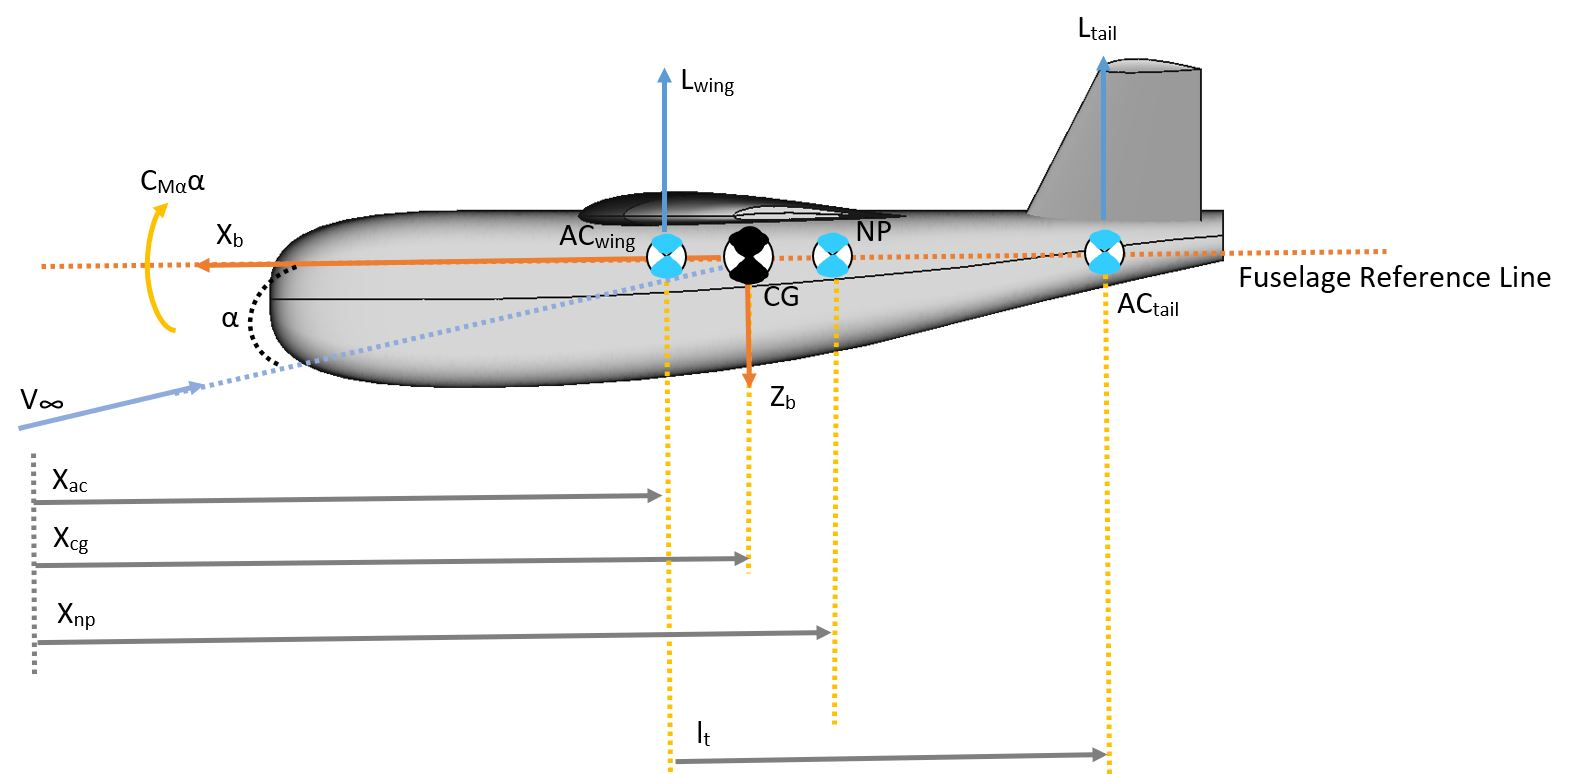
\includegraphics[width=1\linewidth]{03_LiteratureReview/Figs/CGNPAC.JPG}
  \caption{Position of center of gravity (CG), neutral point (NP) and aerodynamic center (AC)}
  \label{fig:AC}
\end{figure}

Another important concept for stability is the static margin. The static margin is defined as the distance between the neutral point and the centre of gravity indicated in Figure \ref{fig:AC}. The static margin is expressed as a percentage of the mean aerodynamic chord length and is given in Equation \ref{eqn:cm}. A large static margin indicates that an aircraft is stable. 

\begin{equation}
    C_{M_\alpha} = C_{L_\alpha} ( \frac{x_{cg}}{\overline{c}} - N_0 )
    \label{eqn:cm}
\end{equation}

If the centre of gravity is positioned too far forward, the pitching stiffness coefficient becomes negative with a large magnitude. Aircraft in this state require large control surface deflections to be manoeuvrable. Aircraft are designed with this stability in mind, and the pitch stiffness is placed within reasonable controllability and stability limitations. Figure \ref{fig:stable} shows the stability difference when moving the center of gravity and neutral point locations. 


\begin{figure}[H]
     \centering
     \begin{subfigure}[b]{0.45\textwidth}
         \centering
         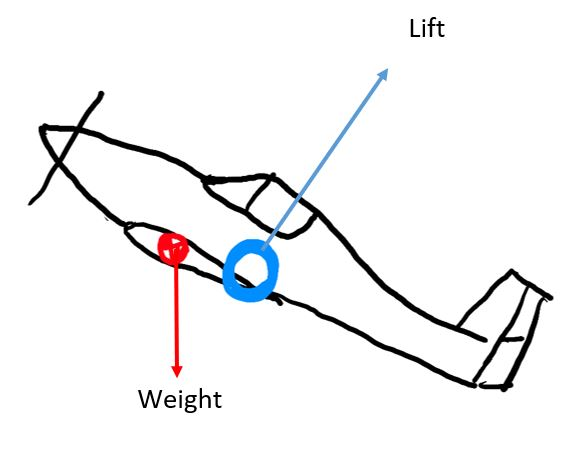
\includegraphics[width=\textwidth]{02_Background/Figs/a3.JPG}
         \caption{When the center of gravity is ahead of the neutral point then the weight tends to correct this displacement (stable).}
         \label{fig:Pressa2a}
     \end{subfigure}
     \hfill
     \begin{subfigure}[b]{0.45\textwidth}
         \centering
         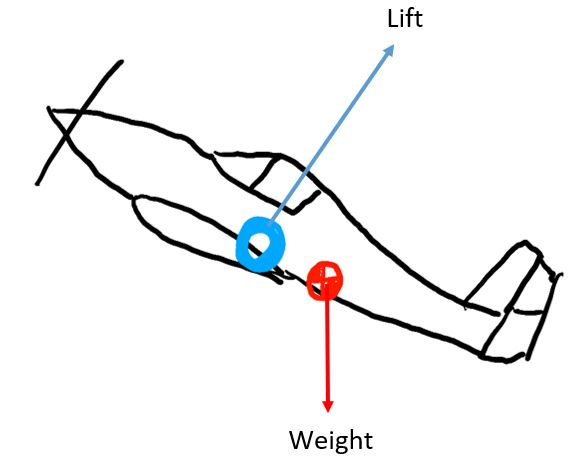
\includegraphics[width=\textwidth]{02_Background/Figs/b3.JPG}
         \caption{When center of gravity is behind the neutral point the weight worsens the displacement (unstable). }
         \label{fig:Pressa2b}
     \end{subfigure}
     \hfill
        \caption{General forces acting through the neutral point and center of gravity for a stable and unstable state}
    \label{fig:stable}
\end{figure}




\section{Static Lateral Stability}

Static lateral stability is determined by the roll moment \textit{L} and yaw moment \textit{N}. Similarly to how the lift and drag coefficients were normalised, the roll and yaw moments can be normalised to form their coefficient forms. These Equations are given in \ref{eqn:roll} and \ref{eqn:yaw}. 

\begin{equation}
    C_L = \frac{L}{\frac{1}{2} \rho {V_\infty}^2 S b }
    \label{eqn:roll}
\end{equation}

\begin{equation}
    C_N = \frac{N}{\frac{1}{2} \rho {V_\infty}^2 S b }
    \label{eqn:yaw}
\end{equation}

The lateral stability of an aircraft is based on the change in $C_N$ and $C_L$ with respect to disturbances in the sideslip angle. A further parameter can be determined from the yaw moment by taking the derivative with respect to the sideslip angle. This is given in Equation \ref{eqn:sideslip}. This is also known as yaw stiffness.

\begin{equation}
    C_{n_\beta} = \frac{\delta C_N}{\delta \beta} > 0
    \label{eqn:sideslip}
\end{equation}


A positive sideslip angle change for directional stability must produce a positive yaw moment change. A positive yaw moment shifts the aircraft to re-align the body and wind axes, reducing the sideslip angle. This is described in Equation \ref{eqn:sideslip}. 

Similarly, the derivative of the roll moment with respect to the sideslip angle can be used to determine the dihedral effect shown in Equation \ref{eqn:dihedral}.

\begin{equation}
    C_{l_\beta} = \frac{\delta C_l}{\delta \beta} < 0
    \label{eqn:dihedral}
\end{equation}
A positive sideslip angle change will produce a negative rolling moment to be laterally stable. This causes an aircraft to roll away from the relative wind flow. Hence a yawing movement to align with the air path is produced. This condition is given in Equation \ref{eqn:dihedral}. 

However, it is possible to have an aircraft that meets these criteria but is still hard to control. If the yaw or roll is too stiff (i.e. $C_{N_\beta}$ is positive with a large magnitude and $C_{L_\beta}$ is negative with a large magnitude), then the aircraft can still become impossible to manoeuvre. Hence the limitations of $C_{N_\beta}$ and $C_{L_\beta}$ are primarily limited by the actual controllability of the aircraft. 




\begin{figure}[H]
% \hspace*{-1.3in}
  \centering
   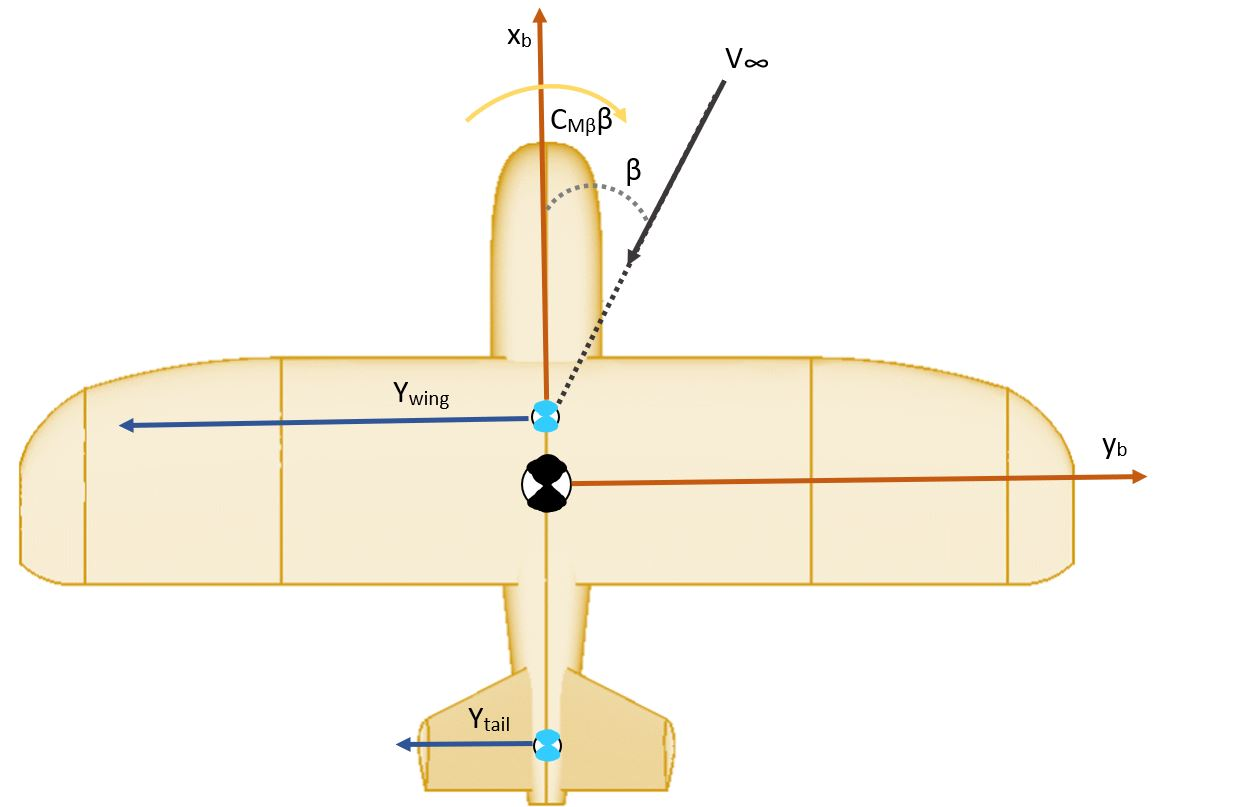
\includegraphics[width=0.8\linewidth]{03_LiteratureReview/Figs/sideslip.JPG}
  \caption{Relevant parameters when an aircraft undergoes a sideslip motion}
  \label{fig:sideslip}
\end{figure}

\begin{figure}[H]
% \hspace*{-1.3in}
  \centering
   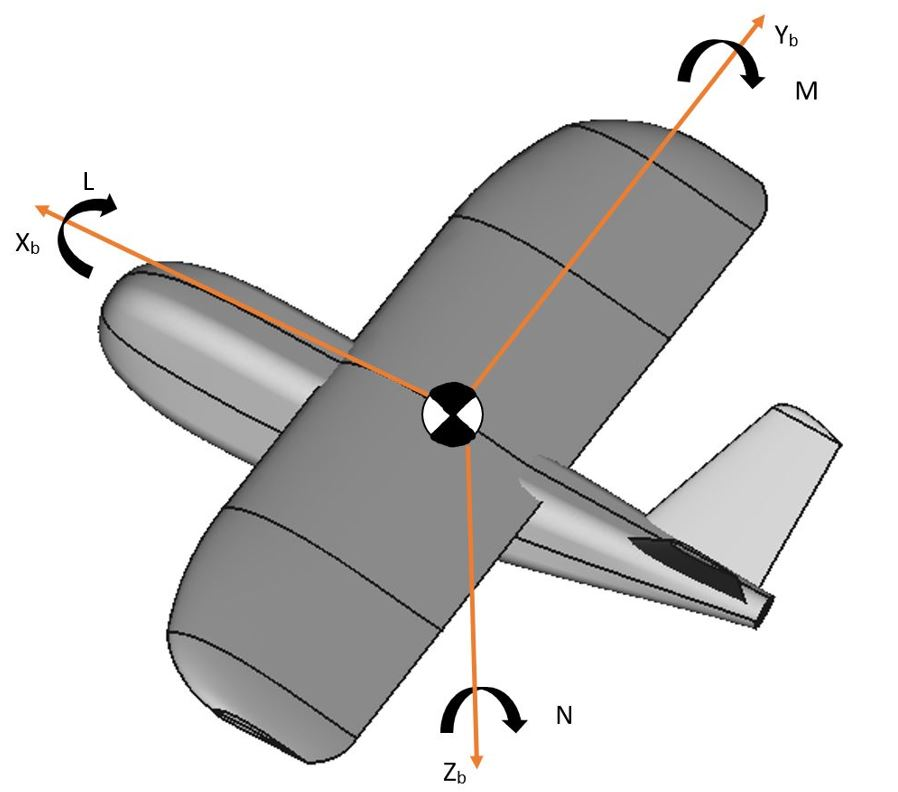
\includegraphics[width=0.8\linewidth]{03_LiteratureReview/Figs/axes2.JPG}
  \caption{Moments acting on an aircraft}
  \label{fig:pitch}
\end{figure}




\section{Reynolds Number}
Reynolds number is a dimensionless number used to represent the ratio of inertial forces to viscous forces. It is expressed in Equation \ref{eqn:reynolds} where:

\begin{itemize}
    \item $\nu$ represents the kinematic viscosity of the fluid.
    \item $\rho$ represents the density of the fluid (air in this case).
    \item u is the flow speed.
    \item L is a characteristic length. In the case of aircraft, this is typically the width of the frontal area being investigated.
    \item $\mu$ is the dynamic viscosity of the fluid.
\end{itemize} 

\begin{equation}
    Re = \frac{\rho uL}{\mu} = \frac{uL}{\nu}
    \label{eqn:reynolds}
\end{equation}

Figure \ref{fig:Repipe} shows a visualisation of these parameters. 

\begin{figure}[H]
    \centering
    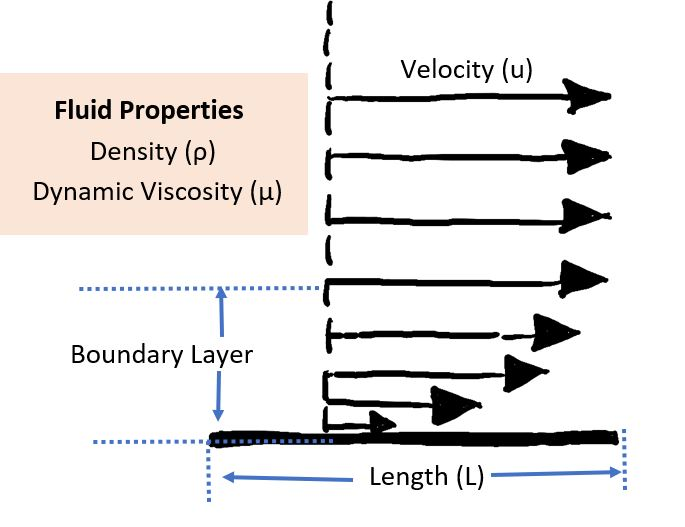
\includegraphics[scale=0.75]{02_Background/Figs/BoundaryLayerUpdated.JPG}
    \caption{Reynolds number parameters when describing the flow over a flat plate}
    \label{fig:Repipe}
\end{figure}

The Reynolds number is a parameter for describing the flow of the fluid being investigated. It is often used when describing flow transitions from laminar to turbulent flow and other general fluid transitions. An example is shown in Figure \ref{fig:Re2}.


\begin{figure}[H]
    \centering
    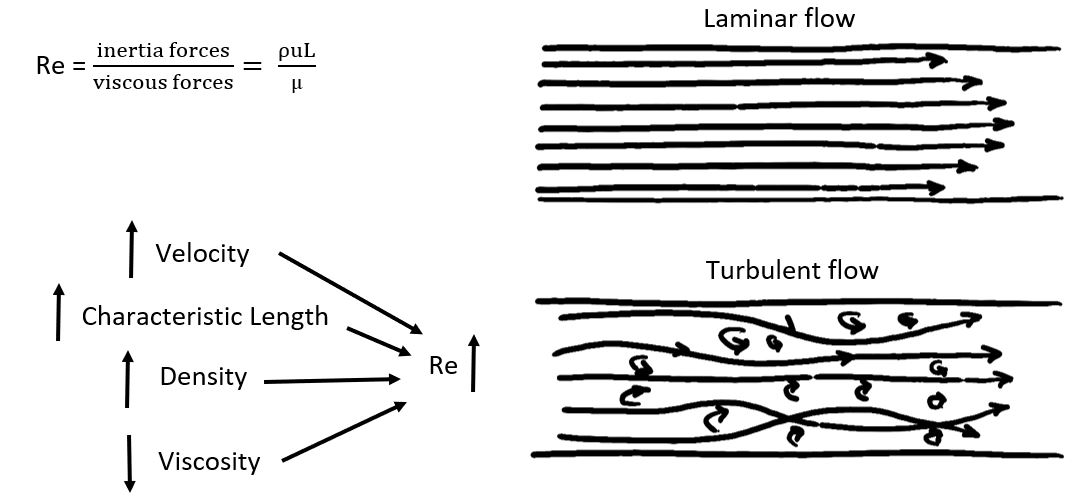
\includegraphics[scale=0.75]{02_Background/Figs/flowType2.JPG}
   \caption{Reynolds number parameters which induce the transition from laminar to turbulent flow}
    \label{fig:Re2}
\end{figure}

% \begin{figure}[H]
%     \centering
%     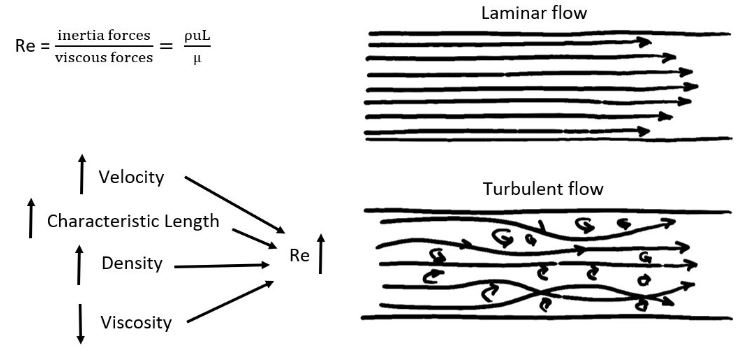
\includegraphics[scale=1\linewidth]{02_Background/Figs/re.JPG}
%     \caption{Reynolds number parameters which induce the transition from laminar to turbulent flow}
%     \label{fig:Re2}
% \end{figure}

High Reynolds values ($> 10^{6}$) indicate that the viscous forces only account for a small amount of the flow and hence the flow is essentially inviscid. For low Reynolds number values ($< 10^{5}$), the viscous forces account for a significant portion of the flow and must be considered.




